\documentclass[10.5pt,scale=1.0,t,aspectratio=169,hyperref={pdfpagelabels=false}]{beamer}
%\usepackage[paperwidth=13.33in, paperheight=7.5in,top=.25in, bottom=.25in, left=.25in, right=.25in]{geometry}
%\geometry{papersize={13.33in,7.5in}}

%\usetheme{Dresden}
%\usetheme{Warsaw}

%Other themes
%https://hartwork.org/beamer-theme-matrix/

\usepackage{lipsum}
\usepackage{color}

\usepackage{amsfonts}
\usepackage{amsmath,mathtools}
\usepackage{mathrsfs}
\usepackage{array}
\usepackage{algorithm}
\usepackage{hyperref}
\usepackage[spanish,es-nodecimaldot]{babel}
\usepackage[utf8]{inputenc}
%\usepackage{intcalc}
\usepackage{graphicx}
\usepackage{multicol}
%\usepackage{authblk}
\usepackage{multirow}
\usepackage{enumitem}
\usepackage[document]{ragged2e}

\usepackage[absolute,overlay]{textpos}
\textblockorigin{0mm}{0mm} 

\usefonttheme[onlymath]{serif}
%\usepackage{epstopdf}
\usepackage{verbatim}
\usepackage{cite}
%\usepackage[texcoord,grid,gridunit=mm,gridcolor=red!10,subgridcolor=green!10]{eso-pic}




\newenvironment{conditions}[1][where:]
{#1 \begin{tabular}[t]{>{$}l<{$} @{${}={}$} l}}
	{\end{tabular}\\[\belowdisplayskip]}


\newcolumntype{L}{>{$}l<{$}} % math-mode version of "l" column type


\newcounter{saveenumi}
\newcommand{\seti}{\setcounter{saveenumi}{\value{enumi}}}
\newcommand{\conti}{\setcounter{enumi}{\value{saveenumi}}}

\setbeamertemplate{bibliography item}{\insertbiblabel}


\hypersetup{colorlinks=true,
	linkcolor=blue,
	linktoc=all,				
	citecolor=blue,
	urlcolor=red,
	pdftitle={FUNDAMENTOS DE AUTOMATIZACIÓN Y CONTROL},
	pdfauthor={Santiago Rúa Pérez},
	pdfcreator={Santiago Rúa Pérez}}


\definecolor{GreenDark}{rgb}{0.0, 0.60, 0.0}
\definecolor{RedDark}{rgb}{183, 0.0, 0.0}
\definecolor{BlueDark}{rgb}{0.0, 0.0, 167}
\definecolor{BlueLight}{rgb}{0.2, 0.451, 0.517}


\graphicspath{{imag/}}

\newcommand{\Ho}{$H_{0}$}
\newcommand{\Ha}{$H_{a}$}
\newcommand{\Nota}{{\bf Nota: }}
\newcolumntype{P}[1]{>{\centering\arraybackslash}p{#1}}
\newcolumntype{M}[1]{>{\centering\arraybackslash}m{#1}}

\newcommand{\less}{<}
\newcommand{\greater}{>}


\setlength{\parindent}{1em}
\setlength{\parskip}{.6em}
\renewcommand{\baselinestretch}{.9}

%%%%    C environment    ---------------- %%%%%%%%%%%%%%%.
\usepackage{listings}
\usepackage{xcolor}
\definecolor{mGreen}{rgb}{0,0.6,0}
\definecolor{mGray}{rgb}{0.5,0.5,0.5}
\definecolor{mPurple}{rgb}{0.58,0,0.82}
\definecolor{backgroundColour}{rgb}{0.95,0.95,0.92}

\lstdefinestyle{CStyle}{
	backgroundcolor=\color{backgroundColour},   
	commentstyle=\color{mGreen},
	keywordstyle=\color{magenta},
	numberstyle=\tiny\color{mGray},
	stringstyle=\color{mPurple},
	basicstyle=\tiny,
	breakatwhitespace=false,         
	breaklines=true,                 
	captionpos=b,                    
	keepspaces=true,                 
	numbers=left,                    
	numbersep=5pt,                  
	showspaces=false,                
	showstringspaces=false,
	showtabs=false,                  
	tabsize=2,
	language=C
}
%%--------------------------------------------------------------------------


\title{Electrónica digital II}   
\author{Santiago Rúa Pérez, PhD.} 
\date{\today} 

\setlength{\TPHorizModule}{\textwidth}
\setlength{\TPVertModule}{\textwidth}

\newcommand{\btVFill}{\vskip0pt plus 1filll}


\setbeamertemplate{sidebar right}{}
\setbeamertemplate{footline}
{
	\leavevmode%
	\hbox{%
		\begin{beamercolorbox}[wd=.333333\paperwidth,ht=2.25ex,dp=1ex,center]{author in head/foot}%
			\usebeamerfont{author in head/foot}\insertshortauthor
		\end{beamercolorbox}%
		\begin{beamercolorbox}[wd=.333333\paperwidth,ht=2.25ex,dp=1ex,center]{title in head/foot}%
			\usebeamerfont{title in head/foot}\insertshorttitle
	\end{beamercolorbox}}%
	\vskip0pt%
}
\makeatother

\begin{document}
	%%%%%%%%%%%%%%%%%% FRAME %%%%%%%%%%%%%%%%%%%%%%%%%%
	\begin{frame}
		\titlepage
	\end{frame}
	%%%%%%%%%%%%%%%%% FRAME START %%%%%%%%%%%%%%%%%%%%%%%%%%
	\frame{
		%\frametitle{}
		\begin{center}
			\LARGE \textcolor{blue}{ARREGLOS EN C}
		\end{center}
		
	}
	%%%%%%%%%%%%%%%%% FRAME START %%%%%%%%%%%%%%%%%%%%%%%%%%
%%%%%%%%%%%%%%%%% FRAME START %%%%%%%%%%%%%%%%%%%%%%%%%%

%%%%%%%%%%%%%%%%% FRAME %%%%%%%%%%%%%%%%%%%%%%%%%%
\begin{frame}
	\frametitle{Arreglos en C}
	{\bf Objetivos}
	\begin{itemize}
	\item Utilizar los arreglos para representar listas o tablas.
	\item Definir un arreglo, inicializarlo y direccionar.
	\item Definir constantes simbólicas.
	\item Pasar arreglos a funciones.
	\item Definir arreglos multidimensionales.
	\item Crear arreglos de longitud variable.
	\end{itemize}
\end{frame}

%%%%%%%%%%%%%%%%% FRAME %%%%%%%%%%%%%%%%%%%%%%%%%%
\begin{frame}
	\frametitle{Arreglos}
	Es un conjunto de datos organizados de forma contigua en memoria.  
	\begin{figure}
		\centering
		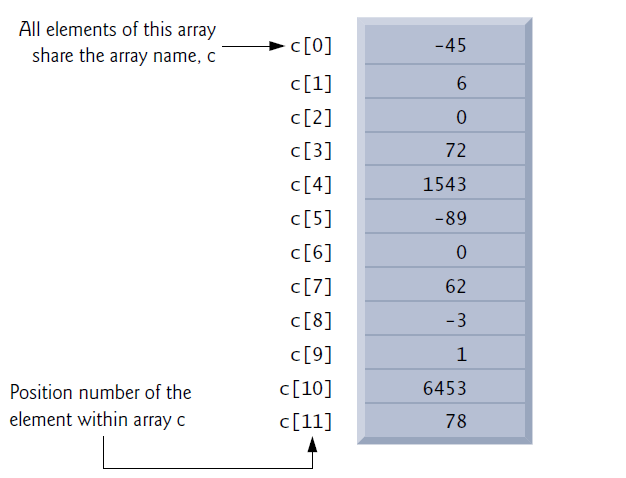
\includegraphics[scale=0.5]{Array}
	\end{figure}
\end{frame}
%%%%%%%%%%%%%%%%% FRAME %%%%%%%%%%%%%%%%%%%%%%%%%%
\begin{frame}[fragile]
	\frametitle{Arreglos - Declaración}
	Para crear un vector basta con indicar el nombre del vector y el tamaño del mismo, de esta forma se le da la orden al compilador el espacio en memoria. 
	\begin{lstlisting}[style=CStyle]
		#include <stdio.h>
		
		// function main begins program execution
		int main(void)
		{
			int n[5]; // n is an array of five integers
			
			// set elements of array n to 0
			for (size_t i = 0; i < 5; ++i) {
				n[i] = 0; // set element at location i to 0
			}
			
			printf("% s% 13s\n", "Element", "Value");
			
			// output contents of array n in tabular format
			for (size_t i = 0; i < 5; ++i) {
				printf("% 7u% 13d\n", i, n[i]);
			}
		}
	\end{lstlisting}
	Pueden inicializarse mediante lista de elementos. También se puede definir la directiva de preprocesamiento \texttt{\#define}. 
\end{frame}
%%%%%%%%%%%%%%%%% FRAME %%%%%%%%%%%%%%%%%%%%%%%%%%
\begin{frame}[fragile]
	\frametitle{Inicialización - Ejemplo} 
	\begin{lstlisting}[style=CStyle]
		#include <stdio.h>
		
		// function main begins program execution
		int main(void)
		{
			// use initializer list to initialize array n
			int n[5] = {32, 27, 64, 18, 95};
			
			printf("%s%13s\n", "Element", "Value");
			
			// output contents of array in tabular format
			for (size_t i = 0; i < 5; ++i) {
				printf("%7u%13d\n", i, n[i]);
			}
		}
	\end{lstlisting}
\end{frame}
%%%%%%%%%%%%%%%%% FRAME %%%%%%%%%%%%%%%%%%%%%%%%%%
\begin{frame}[fragile]
	\frametitle{Inicialización variable simbólica - Ejemplo} 
	\begin{lstlisting}[style=CStyle]
		#include <stdio.h>
		
		#define SIZE 5 // maximum size of array
		
		// function main begins program execution
		int main(void)
		{
			// symbolic constant SIZE can be used to specify array size
			int s[SIZE]; // array s has SIZE elements
			
			for (size_t j = 0; j < SIZE ; ++j) { // set the values
				s[j] = 2 + 2 * j;
			}
			
			printf("%s%13s\n", "Element", "Value");
			
			// output contents of array s in tabular format
			for (size_t j = 0; j < SIZE ; ++j) {
				printf("%7u%13d\n", j, s[j]);
			}
		}
	\end{lstlisting}
\end{frame}
%%%%%%%%%%%%%%%%% FRAME %%%%%%%%%%%%%%%%%%%%%%%%%%
\begin{frame}
	\frametitle{Arreglos - Ejercicio}
	\begin{itemize}
		\item 	Cuarenta estudiantes fueron encuestados sobre la calidad de comida en un restaurante es un escala de 1 a 10 siendo está última como la mejor. Ponga las 40 respuestas en un vector de enteros y encuentre el resumen de los resultados de la encuesta. 
		\item Lance los dados 60000000 de veces y haga un resumen de los resultados.  
		\item Haga un programa que dado un vector de tamaño n, los organice de mayor a menor. 
	\end{itemize} 
\end{frame}

%%%%%%%%%%%%%%%%% FRAME %%%%%%%%%%%%%%%%%%%%%%%%%%
\begin{frame}[fragile]
	\frametitle{Solución primer ejercicio} 
	\begin{lstlisting}[style=CStyle]
		#include <stdio.h>
		
		#define SIZE 5 // maximum size of array
		
		// function main begins program execution
		int main(void)
		{
			// symbolic constant SIZE can be used to specify array size
			int s[SIZE]; // array s has SIZE elements
			
			for (size_t j = 0; j < SIZE ; ++j) { // set the values
				s[j] = 2 + 2 * j;
			}
			
			printf("%s%13s\n", "Element", "Value");
			
			// output contents of array s in tabular format
			for (size_t j = 0; j < SIZE ; ++j) {
				printf("%7u%13d\n", j, s[j]);
			}
		}
	\end{lstlisting}
\end{frame}
%%%%%%%%%%%%%%%%% FRAME %%%%%%%%%%%%%%%%%%%%%%%%%%
\begin{frame}[fragile]
	\frametitle{Cadenas} 
	Las cadenas son un arreglo de caracteres terminados con el valor NULL. El valor NULL se puede representar mediante \verb*|'\0'|. Por ejemplo
	\begin{lstlisting}[style=CStyle]
		char string1[] = "first";
		char string1[] = {'f', 'i', 'r', 's', 't', '\0'};
	\end{lstlisting}
	Ambas cadenas son lo mismo y generan el mismo tamaño.
	
	Para manipular cadenas, existen librerias propias dentro de C especializadas en el tratamiento de las mismas. Un ejemplo de estas funciones son: \verb*|fgets|, \verb*|puts|, \verb*|sscanf|, \verb*|sprintf|, entre otras. 
\end{frame}

%%%%%%%%%%%%%%%%% FRAME %%%%%%%%%%%%%%%%%%%%%%%%%%
\begin{frame}[fragile]
	\frametitle{Enviar arreglos a funciones} 
	Para pasar un arreglo completo a una función se debe enviar el nombre del arreglo sin nada entre corchetes. Automáticamente C detecta que esto es un paso por referencia.
	\begin{multicols}{2} 
	\begin{lstlisting}[style=CStyle]
		#include <stdio.h>
		#define SIZE 5
		
		void modifyArray(int b[], size_t size);
		void modifyElement(int e);
		
		int main(void)
		{
			int a[SIZE] = {0, 1, 2, 3, 4}; // initialize array a
			
			puts("Effects of passing entire array by reference:\n\nThe values of the original array are:");
			
			for (size_t i = 0; i < SIZE; ++i) {
				printf("% 3d", a[i]);
			}
			
			puts(""); // outputs a newline
			modifyArray(a, SIZE); // pass array a to modifyArray by reference
			puts("The values of the modified array are:");
			
			// output modified array
			for (size_t i = 0; i < SIZE; ++i) {
				printf("% 3d", a[i]);
			}
			
			printf("\n\n\nEffects of passing array element by value:\n\nThe value of a[3] is %d\n", a[3]);
			modifyElement(a[3]); // pass array element a[3] by value
			printf("The value of a[3] is % d\n", a[3]);
		}
		
		void modifyArray(int b[], size_t size)
		{
			for (size_t j = 0; j < size; ++j) {
				b[j] *= 2; // actually modifies original array
			}
		}
		void modifyElement(int e)
		{
			printf("Value in modifyElement is % d\n", e *= 2);
		}
	\end{lstlisting}
\end{multicols}
\end{frame}
%%%%%%%%%%%%%%%%% FRAME %%%%%%%%%%%%%%%%%%%%%%%%%%
\begin{frame}
	\frametitle{Tarea} 
	\begin{itemize}
		\item Consultar como funciona el algoritmo de ordenamiento de burbuja.
		\item Consultar como funciona la busqueda lineal vs la busqueda binaria en un arreglo.
	\end{itemize}
\end{frame}
%%%%%%%%%%%%%%%%% FRAME %%%%%%%%%%%%%%%%%%%%%%%%%%
\begin{frame}[fragile]
	\frametitle{Arreglos - Multidimensionales}
	Un arreglo multidimensional consiste en formar un vector de vectores. 
	\begin{figure}
		\centering
		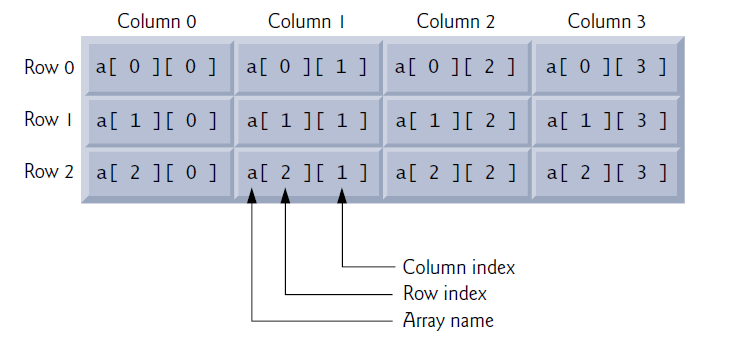
\includegraphics[scale=0.7]{Matriz}
	\end{figure}
	La inicialización se realizar indicando las dos dimensiones entre dos corchetes para las filas y columnas. Asi
	\begin{lstlisting}[style=CStyle]
	int b[2][2] = {{1}, {3, 4}};
	\end{lstlisting}
	
\end{frame}
%%%%%%%%%%%%%%%%% FRAME %%%%%%%%%%%%%%%%%%%%%%%%%%
\begin{frame}[fragile]
	\frametitle{Arreglos - Multidimensionales - Ejemplo}
	\begin{multicols}{2} 
	\begin{lstlisting}[style=CStyle]
		#include <stdio.h>
		
		void printArray(int a[][3]); // function prototype
		
		// function main begins program execution
		int main(void)
		{
			int array1[2][3] = {{1, 2, 3}, {4, 5, 6}};
			puts("Values in array1 by row are:");
			printArray(array1);
			
			int array2[2][3] = {1, 2, 3, 4, 5};
			puts("Values in array2 by row are:");
			printArray(array2);
			
			int array3[2][3] = {{1, 2}, {4}};
			puts("Values in array3 by row are:");
			printArray(array3);
		}
		
		// function to output array with two rows and three columns
		void printArray( int a[][3])
		{
			// loop through rows
			for (size_t i = 0; i <= 1; ++i) {
				// output column values
				for (size_t j = 0; j <= 2; ++j) {
					printf("% d ", a[i][j]);
				}
				printf("\n"); // start new line of output
			}
		}
	\end{lstlisting}
	\end{multicols}

El compilador necesita saber cuantos elementos hay en cada fila, por eso se requiere mandar el dato de las columnas cuando se hace el llamado a la función. 
\end{frame}
%%%%%%%%%%%%%%%%% FRAME %%%%%%%%%%%%%%%%%%%%%%%%%%
\begin{frame}
	\frametitle{Arreglos - Multidimensionales - Ejemplo}
	Implemente un programa que dado una matriz de notas de estudiantes, obtenga la menor nota, la mayor nota, y el promedio de cada estudiante. 
	
	\begin{figure}
		\centering
		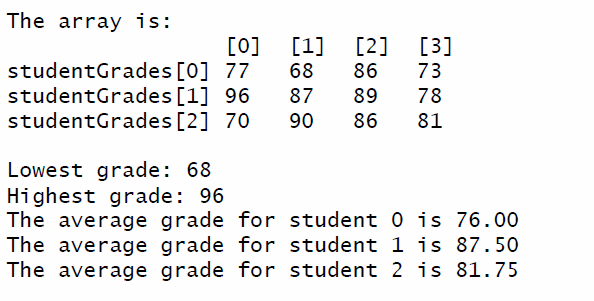
\includegraphics[scale=0.7]{EjemploNotas}
	\end{figure}
\end{frame}
%%%%%%%%%%%%%%%%% FRAME %%%%%%%%%%%%%%%%%%%%%%%%%%
\begin{frame}
	\frametitle{Arreglos - Longitud Variable}
	Son arreglos cuyo tamaño se elige en tiempo de ejecución y no en tiempo de compilación (Caracteristica no soportada en Microsoft Visual C++).  
\end{frame}
%%%%%%%%%%%%%%%% FRAME %%%%%%%%%%%%%%%%%%%%%%%%%%
\frame{
\begin{center}
	\LARGE \textcolor{blue}{ARREGLOS EN C}
\end{center}

\begin{center}
	\LARGE \textcolor{blue}{GRACIAS}
\end{center}
}

%%%%%%%%%%%%%%%%%%%%%%%%%%%%%%%%%%%%%%%%%%%%%%%%%%%%%%%%%%%%%%%%%%%%%%%%%%%%%%%%%%%%%%%%%%%%%%%%%%%%%%%%%%%%%



\end{document}

